\documentclass[letterpaper,11pt,twoside]{article}
\usepackage{amsmath,amssymb,amsfonts,amsthm}
\usepackage[margin=1.0in]{geometry}
\usepackage{fancyhdr, lastpage}
\usepackage[pdftex]{graphicx}
\usepackage{hyperref}
\hypersetup{
    colorlinks,
    citecolor={black},
    linkcolor={black},
    urlcolor={black},
    bookmarksnumbered,
    pdfstartview={FitH},
    pdfpagemode={UseOutlines},
    pdftitle={Project Report - Distributed Query Processing},
    pdfauthor={Larry Bowers, James Bradwell, Evan Dickinson, Bhadresh Patel, and Lewis Pearson},
    pdfsubject={CS 453 Project Report}
}

\setlength{\parskip}{0.5ex}
\pagestyle{fancy}
\setlength{\headheight}{14.0pt}
\fancyhead{}
\fancyfoot{}
\fancyhead[RO,RE] {Project Report: \emph{Distributed Query Processing}}
\fancyfoot[LO,LE] {CS 453: Project 4}
\fancyfoot[RO,RE] {Page \thepage\ of \pageref{LastPage}}
\renewcommand{\headrulewidth}{0.5pt}
\renewcommand{\footrulewidth}{0.5pt}

\begin{document}

%%%%%%%%%% Title Page %%%%%%%%%%%%%%%%%%%%%%%%%%%%%%%%%%%%%%%%%%%%%%%%%%%%%%%%%%
\begin{titlepage}
   \begin{center}
       {\Large \textbf{Project Report}}\\[0.5cm]
       {\Large \textbf{CS 453: Project 4}}\\[3.0cm]

       {\rule{\linewidth}{0.5mm}} \\[0.5cm]
       {\Huge \textbf{Distributed Query Processing}}\\[0.4cm] 
       {\rule{\linewidth}{0.5mm}} \\[2.0cm]

       \textbf{Larry Bowers}\\
       \texttt{killergift@wsu.edu}\\[0.5cm]
       \textbf{James Bradwell}\\
       \texttt{jebradwell@gmail.com}\\[0.5cm]
       \textbf{Evan Dickinson}\\
       \texttt{evan13579b@wsu.edu}\\[0.5cm]
       \textbf{Bhadresh Patel}\\
       \texttt{bhadresh@wsu.edu}\\[0.5cm]
       \textbf{Lewis Pearson}\\
       \texttt{lewis\_pearson@wsu.edu}\\[0.5cm]

       \vfill
       Washington State University Vancouver\\
       December 05, 2010
   \end{center}
\end{titlepage}

\begin{abstract}

\end{abstract}

\section{Overview}

\begin{figure}[htb]
 \centering
 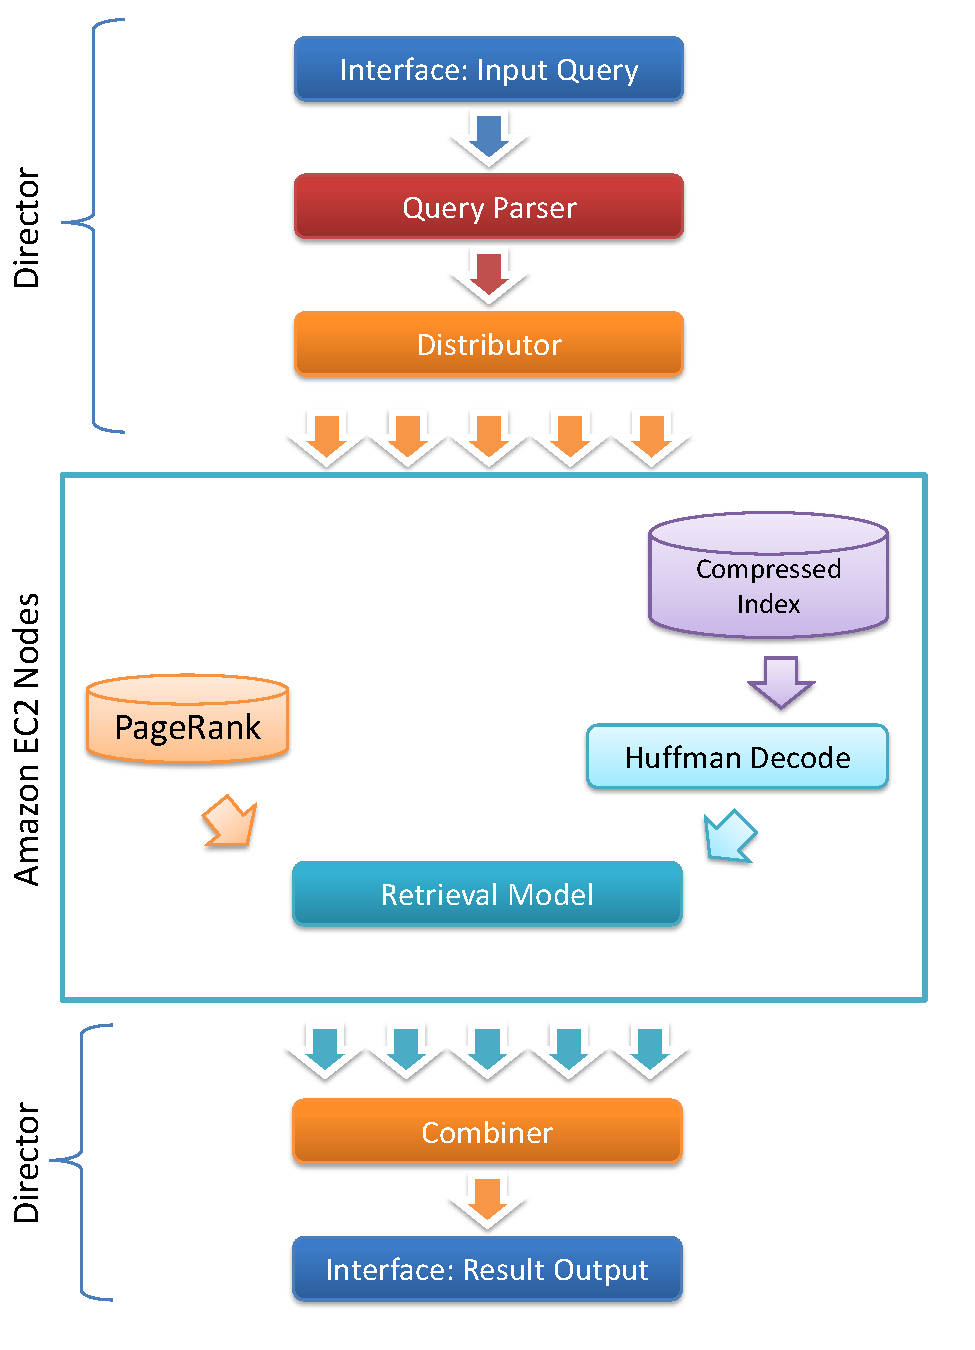
\includegraphics[trim=0.0in 0.00in 0.0in 0.0in, clip, page=1]{Architecture.pdf}
 \caption{Architecture Overview}
 \label{fig:Architecture}
\end{figure}

\section{Interface}

\subsection{Query Input}

\subsection{Result Output}

\section{Distributed Evaluation}

\subsection{Distributer}

\subsection{Index Server}

\subsection{Merge Results}

\section{Index Compression}


\section{Reterival Model}


\section{Roles}
\begin{description}
  \item[Larry Bowers] User interface and query parser
  \item[James Bradwell] User interface and query parser
  \item[Evan Dickinson] Huffman encoding/decoding 
  \item[Bhadresh Patel] Distributed processing
  \item[Lewis Pearson] Reterival model
\end{description}

\section{Test Environment}


\section{Usage Guide}


\end{document}
